A Passive Daytime Radiative Cooling (PDRC) device operates by absorbing a lower amount of radiation than it emits, thereby facilitating electricity-free cooling, even in daylight conditions. Consequently, one of the pivotal attributes of a PDRC device is the imperative for an absorptivity ($\alpha$) as close to 0\% or, conversely, a reflectivity ($R$) of 100\% within the solar spectrum (ranging from 0.3 to 2.5 micrometers). This specification ensures that the device's surface remains entirely unaffected by solar heating during daylight hours. Additionally, it is critical that the device exhibits an emissivity or absorptivity close to 100\% over long wavelengths, particularly within the atmospheric window (ranging from 8 to 13 micrometers), to maximize thermal radiation emission back into space. In this wavelength range, the device's reflectivity should be nearly 0\%, which further enhances its cooling efficiency by minimizing the absorption of Earth-emitted radiation, thereby optimizing the device for passive cooling under direct sunlight. See figure \ref{fig:ideal_PDRC_properties_copy} for these ideal properties.

\begin{figure}[ht!]
  \centering
  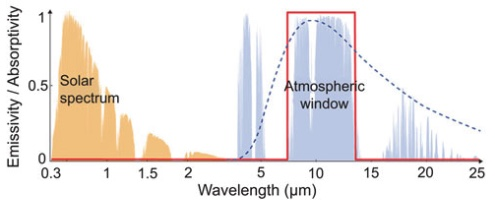
\includegraphics[width=0.4\textwidth]{Chapters/Figures/Chapter 2 Figures/Ideal Optical Properties of a Radiative Cooling Surface copy.jpg}
  \caption[Ideal Optical Properties of a Radiative Cooling Surface]{Ideal Optical Properties of a Radiative Cooling Surface. Source: \cite{yang_passive_2020}}
  \label{fig:ideal_PDRC_properties_copy}
\end{figure}

To enhance the effectiveness of PDRC, it becomes essential to optimize this reflectivity ($R$) spectrum. One approach for achieving this goal is to perceive light as an electromagnetic wave, and from this perspective, ultimately derive $R$ through the renowned \textit{Fresnel equations}.

The Fresnel equations are mathematical expressions that delineate the proportion of incident electromagnetic fields that is either transmitted or reflected at the interface of two materials with differing refractive indices. This concept aligns precisely with our objectives, as we plan to stack plane surfaces featuring distinct reflective properties and refractive indices. This chapter serves as an exploration of the theoretical framework underpinning the derivation of $R$ via the Fresnel Equations, delving into associated phenomena such as total internal reflection. Additionally, we explore the practical application of these principles to PDRC devices.

\section{Fresnel Equations}
Consider a light ray incident at point P upon a planar interface, leading to the generation of both reflected and refracted rays. It is important to recognize that the refractive index before the interface ($n_1$) and after the interface ($n_2$). are properties intrinsic to the materials themselves, determining how light propagates through them. Specifically, $n_1$ is the refractive index of the material through which the incident and reflected rays travel, while $n_2$ is the refractive index of the material through which the refracted ray travels. The plane of incidence, lying within the x-z plane, is defined by both the surface normal and the direction of the incident ray. See figure \ref{fig:The TE Set-up}.

% inserting the TE wave example
\begin{figure}[ht!]
  \centering
  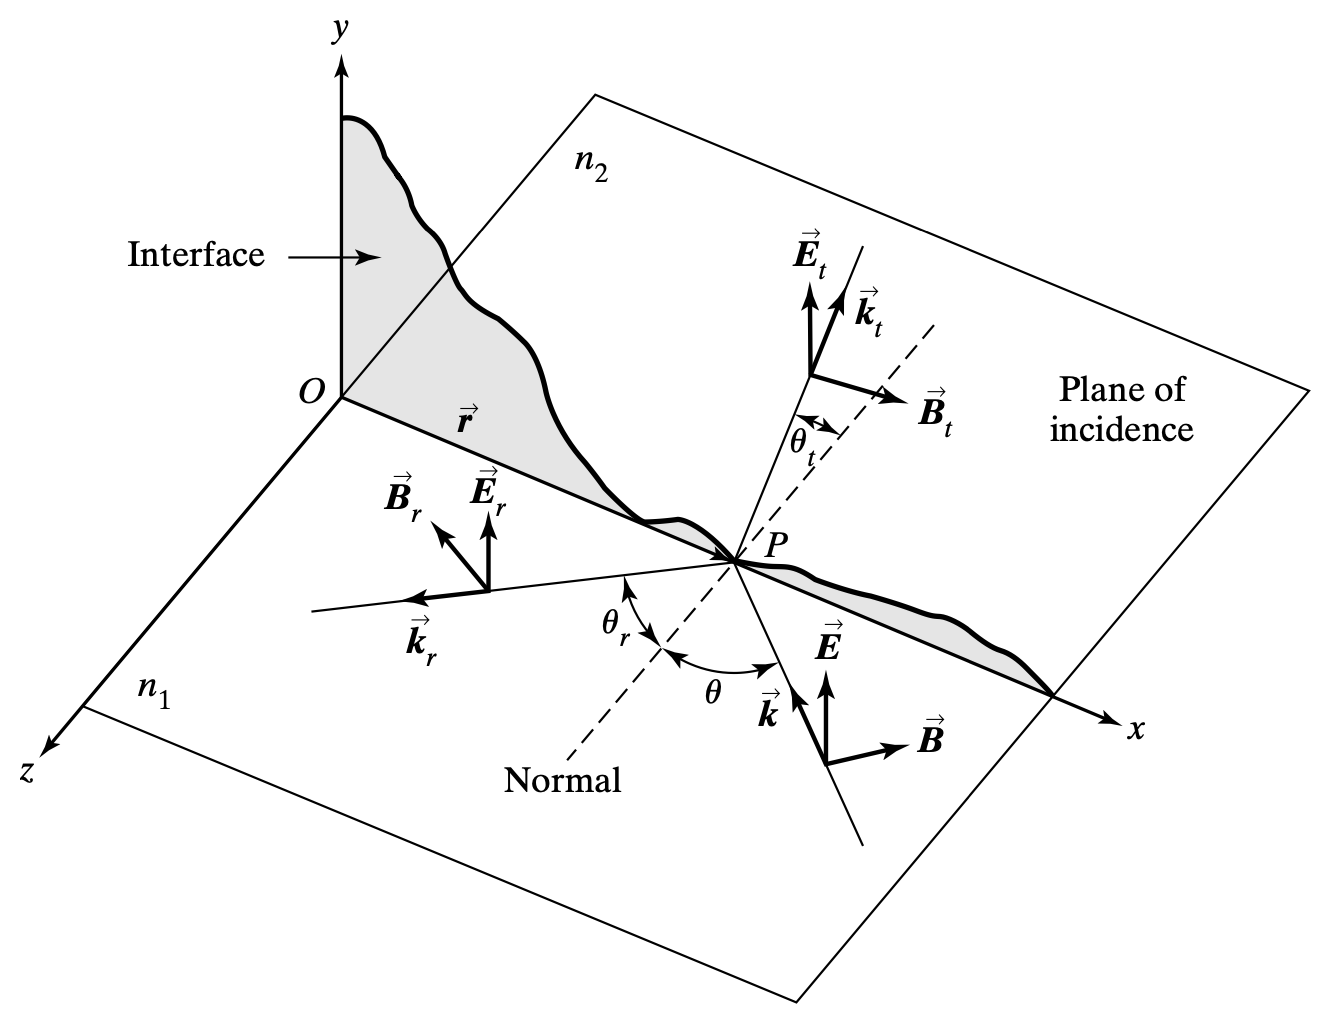
\includegraphics[width=0.8\textwidth]{Chapters/Figures/Chapter 2 Figures/Incident, Reflected, and Transmitted Ray for TE Mode.png}
  \caption[The transverse electric (TE) set-up]{The transverse electric (TE) set-up. Source: \cite{pedrotti_introduction_2007}}
  \label{fig:The TE Set-up}
\end{figure}

In the context of each ray, the direction of wave propagation ($\vec{\mathbf{k}}$), can be established by the vector cross product of the electric field ($\vec{\mathbf{E}}$), and magnetic field ($\vec{\mathbf{B}}$) vectors, expressed as $\vec{\mathbf{E}} \times \vec{\mathbf{B}}$. This relationship can be conveniently determined using the right-hand rule, offering a valuable method for directional assessment.

Let us consider that the incident light comprises of plane harmonic waves:
\begin{equation} \label{Plane harmonic wave equation - incident}
\vec{\mathbf{E}} = \vec{\mathbf{E}_0} e^{i(\vec{\mathbf{k}} \cdot \vec{\mathbf{r}} - \omega t)}
\end{equation}

where 
\begin{itemize}
    \item $\vec{\mathbf{E}}$ represents the electric field vector of the wave at any point.
    \item $\vec{\mathbf{E}_0}$ is the amplitude of $\vec{\mathbf{E}}$ which represents the maximum strength or value of $\vec{\mathbf{E}}$.
    \item $\vec{\mathbf{k}}$ is the wave (direction) vector and it indicates the direction of wave propagation and has a magnitude equal to the wave number $k=\frac{2\pi}{\lambda}$.
    \item $\vec{\mathbf{r}}$ represents the position vector in space where the field is being examined.
    \item $\omega$ is the angular frequency of the wave.
    \item $t$ represents the time.
    \item $i$, the imaginary number, indicates the wave has both real and imaginary components.
\end{itemize}

In our analytical approach, we will specifically examine a linearly polarized light wave, where the electric field vector $\vec{\mathbf{E}}$ is oriented perpendicular to the plane of incidence. According to the right-hand rule, this configuration places the magnetic field vector $\vec{\mathbf{B}}$ within the plane of incidence. This particular polarization is known as the \textit{transverse electric} (TE) mode

The reflected and transmitted waves can then be expressed as plane harmonic waves:
\begin{equation} \label{Plane harmonic wave equation - reflected}
\vec{\mathbf{E}_r} = \vec{\mathbf{E}_{0r}} e^{i(\vec{\mathbf{k_r}} \cdot \vec{\mathbf{r}} - \omega_r t)}
\end{equation}

\begin{equation} \label{Plane harmonic wave equation - refracted}
\vec{\mathbf{E}_t} = \vec{\mathbf{E}_{0t}} e^{i(\vec{\mathbf{k_t}} \cdot \vec{\mathbf{r}} - \omega_t t)}
\end{equation}

where
\begin{itemize}
    \item $\vec{\mathbf{E}_r}$ represents the electric field vector of the reflected wave at any point.
    \item $\vec{\mathbf{E}_t}$ represents the electric field vector of the transmitted wave at any point.
    \item $\vec{\mathbf{k}_r}$ is the wave (direction) vector of the reflected wave.
    \item $\vec{\mathbf{k}_t}$ is the wave (direction) vector of the transmitted wave.
\end{itemize}

% --- SUBSECTION ON BOUNDARY CONDITIONS FOR TE WAVES ---
\subsection{Boundary Conditions for TE Waves}
At the interface where all three waves emerge simultaneously, a crucial boundary condition must be established to govern the relationship between their respective wave amplitudes. This boundary condition stipulates that the waves both incident upon and emerging from the plane of incidence should exhibit continuity and differentiability. This requirement is contingent upon the assumption that the interface is isotropic meaning that the physical properties of the material do not vary with different directions of measurement at the interface.
% Simply put, the condition of the interface being isotropic ensures that the wave will behave the same way regardless of the direction from which it approaches or into which it travels after interacting with the interface.

\begin{equation} \label{Plane harmonic wave equation - reflected}
\vec{\mathbf{E}_r} = \vec{\mathbf{E}_{0r}} e^{i(\vec{\mathbf{k_r}} \cdot \vec{\mathbf{r}} - \omega_r t)}
\end{equation}

In the context of our TE mode configuration (see figure \ref{fig:The TE Set-up}), we can express the waves for the incident, reflected, and transmitted electric field components waves as follows:
    \begin{align*}
    \vec{\mathbf{E}} &= E \hat{y} e^{i(\vec{\mathbf{k}} \cdot \vec{\mathbf{r}} - \omega t)}           &  \vec{\mathbf{E}_r} &= E_r \hat{y} e^{i(\vec{\mathbf{k_r}} \cdot \vec{\mathbf{r}} - \omega_r t)}               &  \vec{\mathbf{E}_t} &= E_t \hat{y} e^{i(\vec{\mathbf{k_t}} \cdot \vec{\mathbf{r}} - \omega_t t)}
    \end{align*}
where $E$, $E_r$, and $E_t$ denote the complex field amplitudes corresponding to the incident, reflected, and transmitted waves, respectively. These waves adhere to the boundary conditions, ensuring the continuity of electric field components parallel to the interface, as in:
\begin{equation} \label{Electric field boundary conditions for TE waves}
E + E_r = E_t
\end{equation}

Using basic trigonometry and Maxwell's equations, we can derive the corresponding magnetic fields for the incident, reflected, and transmitted waves. The expressions for these fields, assuming a TE mode, are:
\begin{align*} 
\vec{\mathbf{B}} &= (B\mathrm{cos}(\theta \hat{x}) - B\mathrm{sin}(\theta \hat{z})) e^{i(\vec{\mathbf{k}} \cdot \vec{\mathbf{r}} - \omega t)} \\
\vec{\mathbf{B}}_r &= (-B_r\mathrm{cos}(\theta_r \hat{x}) - B_r\mathrm{sin}(\theta_r \hat{z})) e^{i(\vec{\mathbf{k_r}} \cdot \vec{\mathbf{r}} - \omega t)} \\ 
\vec{\mathbf{B}}_t &= (B_t\mathrm{cos}(\theta_t \hat{x}) - B_t\mathrm{sin}(\theta_t \hat{z})) e^{i(\vec{\mathbf{k_t}} \cdot \vec{\mathbf{r}} - \omega t)}
\end{align*}

where
\begin{itemize}
    \item $\theta$ represents the angle of incidence (the angle between the incident wave's direction of propagation and the normal to the interface). See figure \ref{fig:The TE Set-up}.
    \item $\theta_r$ represents the angle of reflection (the angle between the reflected wave's direction of propagation and the normal to the interface).
    \item $\theta_t$ represents the angle of transmission (the angle between the transmitted wave's direction of propagation and the normal to the interface).
\end{itemize}

As the magnetic field vector lies transversely to the plane of incidence, adherence to the boundary conditions necessitates the connection of parallel components of the magnetic field, as defined by:
\begin{equation} \label{Magnetic field boundary conditions for TE waves}
B\mathrm{cos}(\theta) - B_r\mathrm{cos}(\theta) = B_t\mathrm{cos}(\theta_t) 
\end{equation}
Here, it's important to note that $\theta = \theta_r$ according to the Law of Reflection. Equations \ref{Electric field boundary conditions for TE waves} and \ref{Magnetic field boundary conditions for TE waves} stand as two pivotal equations arising from the boundary conditions for TE waves. These equations, instrumental in determining $R$, serve as a critical foundation. Nevertheless, before we delve into the calculation of $R$ through these boundary conditions, it is imperative to demonstrate the applicability of the same procedure to the transverse magnetic case.

\subsection{Boundary Conditions for TM Waves}
Another polarization mode for electromagnetic waves is known as the \textit{transverse magnetic} (TM) polarization. In this mode, the magnetic field vector is oriented perpendicular to the plane of incidence, while the electric field vector lies transverse to the plane of incidence. Within the framework of our TM mode configuration, we can formulate the wave equations governing the electric field components of the incident, reflected, and transmitted waves as follows (see figure \ref{fig: The TM set-up}):

% inserting the TM wave example
\begin{figure}[ht!]
  \centering
  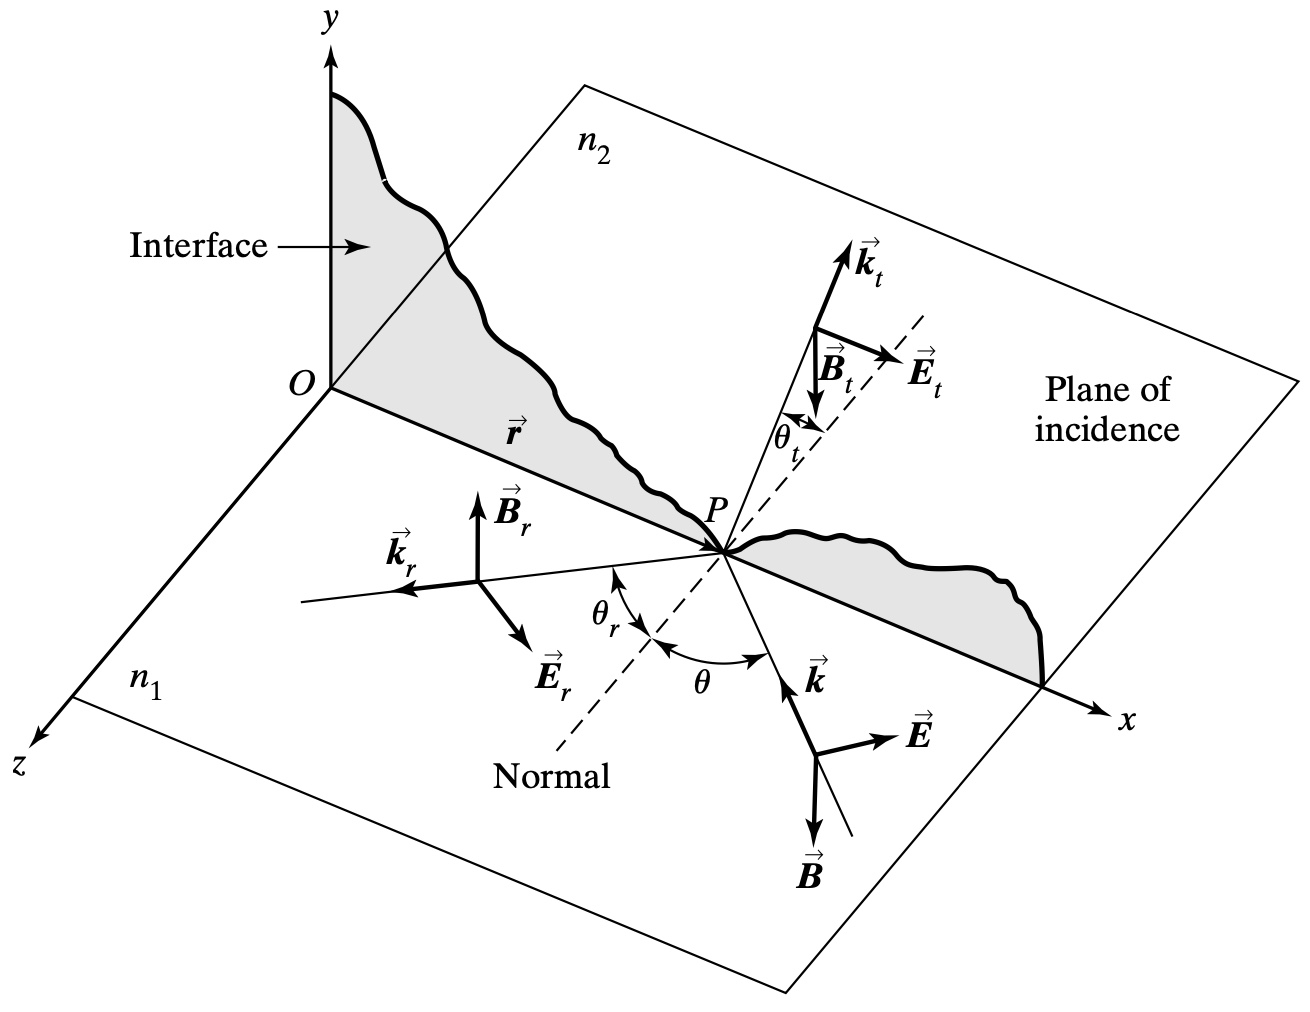
\includegraphics[width=0.8\textwidth]{Chapters/Figures/Chapter 2 Figures/Incident, Reflected, and Transmitted Ray for TM Mode.jpg}
  \caption[The transverse electric (TM) set-up]{The transverse electric (TM) set-up. Source: \cite{pedrotti_introduction_2007}}
  \label{fig: The TM set-up}
\end{figure}

\begin{align*} 
\vec{\mathbf{E}} &= (E\mathrm{cos}(\theta \hat{x}) - E\mathrm{sin}(\theta \hat{z})) e^{i(\vec{\mathbf{k}} \cdot \vec{\mathbf{r}} - \omega t)} \\
\vec{\mathbf{E}}_r &= (E_r\mathrm{cos}(\theta_r \hat{x}) + E_r\mathrm{sin}(\theta_r \hat{z})) e^{i(\vec{\mathbf{k_r}} \cdot \vec{\mathbf{r}} - \omega t)} \\ 
\vec{\mathbf{E}}_t &= (E_t\mathrm{cos}(\theta_t \hat{x}) - E_t\mathrm{sin}(\theta_t \hat{z})) e^{i(\vec{\mathbf{k_t}} \cdot \vec{\mathbf{r}} - \omega t)}
\end{align*}

Consequently, the magnetic field components can be written as (see figure \ref{fig: The TM set-up}):
\begin{align*}
    \vec{\mathbf{B}} &= -B\hat{y} e^{i(\vec{\mathbf{k}} \cdot \vec{\mathbf{r}} - \omega t)} \\
    \vec{\mathbf{B}}_r &= B_r\hat{y} e^{i(\vec{\mathbf{k}} \cdot \vec{\mathbf{r}} - \omega t)} \\
    \vec{\mathbf{B}}_t &= -B_t\hat{y} e^{i(\vec{\mathbf{k_t}} \cdot \vec{\mathbf{r}} - \omega t)} \\
\end{align*}

These equations adhere to the boundary conditions, guaranteeing the continuity of electric field components parallel to the interface, as demonstrated by:
\begin{equation} \label{Magnetic field boundary conditions for TM waves}
-B + B_r = -B_t
\end{equation}

\begin{equation} \label{Electric field boundary conditions for TM waves}
Ecos(\theta) + E_rcos(\theta) = E_tcos(\theta_t)
\end{equation}

% REFLECTION AND TRANSMISSION COEFFICIENTS
\subsection{Reflection and Transmission Coefficients}
To determine the reflectance $R$ and, consequently, the transmittance $T$, it is imperative to define the reflection ($r$) and transmission coefficients ($t$), as follows:
\begin{equation} \label{Definition of the reflection coefficient}
r \equiv \frac{E_r}{E}
\end{equation}
and
\begin{equation} \label{Definition of the transmission coefficient}
t \equiv \frac{E_t}{E}.
\end{equation}

% However, it is essential to calculate these coefficients for both the TE and TM cases. Recall that the electric and magnetic field amplitudes are linked through the following relation:
% \begin{equation} \label{Equation relating the electric and magnetic field amplitudes}
% E = \nu B = \left(\frac{c}{n}\right)B
% \end{equation}
However, it is essential to calculate these coefficients for both the Transverse Electric (TE) and Transverse Magnetic (TM) polarization cases. Recall that the electric (E) and magnetic (B) field amplitudes are interconnected through the following relation:

\begin{equation} \label{Equation relating the electric and magnetic field amplitudes}
E = \nu B = \left(\frac{c}{n}\right)B
\end{equation}

where:
\begin{itemize}
    \item E represents the amplitude of the electric field.
    \item $\nu$ represents the phase velocity of the wave within the medium, $\nu=\frac{c}{n}$.
    \item $n$ is the refractive index of the medium.
    \item $c$ is the speed of light.
\end{itemize}

We can employ \ref{Equation relating the electric and magnetic field amplitudes} to replace every occurrence of $B$ in the boundary conditions with its corresponding $E$. Initiating with the TE case, remember the two vital boundary condition equations for the TE mode:
\begin{equation}
TE:
\begin{cases} \label{TE boundary conditions}
  E + E_r = E_t \\
  n_1Ecos(\theta) - n_1E_rcos(\theta) = n_2E_tcos(\theta_t)
\end{cases}
\end{equation}
We can proceed to solve the system of equations above for the TE case to determine $r_{TE}$ (by eliminating all instances of $E_t$). Introducing the concept of the \textit{relative refractive index}, denoted as $n$ and defined as $n \equiv \frac{n_2}{n_1}$ where $n_1$ is the refractive index of the initial medium through which the incident wave travels, and $n_2$ is the refractive index of the second medium into which the wave is transmitted.

We can derive:
\begin{equation} \label{Reflection coefficient (TE) in terms of n}
r_{TE} = \frac{E_r}{E} = \frac{cos(\theta) - ncos(\theta_t)}{cos(\theta) + ncos(\theta_t)}.
\end{equation}
By the Law of Refraction, $sin(\theta) = nsin(\theta_t)$, so we can eliminate $\theta_t$ by noting that:
\begin{equation} \label{Replacing \theta_t using the law of refraction}
ncos(\theta_t) = n \sqrt{cos^{2}(\theta_t)} = n\sqrt{1 - sin^2(\theta_t)} = \sqrt{n^2 - sin^2(\theta)}
\end{equation}
Finally, our reflection coefficient is:
\begin{equation} \label{eq:reflection_TE}
r_{TE} = \frac{E_r}{E} = \frac{cos(\theta) - \sqrt{n^2 - sin^2(\theta)}}{cos(\theta) + \sqrt{n^2 - sin^2(\theta)}}
\end{equation}

Likewise, employing our boundary conditions for the TM case along with \ref{Equation relating the electric and magnetic field amplitudes}, we arrive at the reevaluated boundary conditions for the TM mode, which are as follows:
\begin{equation}
TM:
\begin{cases} \label{TM boundary conditions}
  -n_1E + n_1E_r = -n_2E_t \\
  Ecos(\theta) + E_rcos(\theta) = E_tcos(\theta_t)
\end{cases}
\end{equation}
With this revised form of the boundary condition, we can compute $r_{TM}$ in a manner similar to our determination of $r_{TE}$, resulting in:
\begin{equation} \label{eq:reflection_TM}
r_{TM} = \frac{E_r}{E} = \frac{-n^2cos(\theta) + \sqrt{n^2 - sin^2(\theta)}}{n^2cos(\theta) + \sqrt{n^2 - sin^2(\theta)}}
\end{equation}
Similarly, if we follow the same steps we did for evaluating $r_{TM}$ and $r_{TE}$, we can subsequently figure out $t_{TM}$ and $t_{TE}$ (we now eliminate $E_r$ instead of $E_t$ ). We find:
\begin{equation} \label{Final tTE}
t_{TE} = \frac{E_t}{E} = \frac{2cos(\theta)}{cos(\theta) + \sqrt{n^2 - sin^2(\theta)}}
\end{equation}

\begin{equation} \label{Final tTM}
t_{TM} = \frac{E_t}{E} = \frac{2ncos(\theta)}{n^2cos(\theta) + \sqrt{n^2 - sin^2(\theta)}}
\end{equation}

Observing, for instance, the interconnection between $t_{TE}$ and $r_{TE}$, it is evident that they share the same denominator, suggesting that one can be expressed in terms of the other. To establish the relationship between the two equations, one can subtract $r_{TE}$ from $t_{TE}$, yielding 1. With some additional manipulation, the corresponding equation linking $t_{TM}$ and $r_{TM}$ can be derived. Ultimately, $r$ can be expressed in terms of $t$ as follows (see figure \ref{fig: The TM set-up}):
\begin{align*}
    t_{TE} &= 1 + r_{TE} \\
    nt_{TM} &= 1 - r_{TM} \\
\end{align*}

The set of equations $r_{TE}$ (\ref{eq:reflection_TE}), $r_{TM}$ (\ref{eq:reflection_TM}), $t_{TE}$ (\ref{Final tTE}), and $t_{TM}$ (\ref{Final tTM}) constitutes the \textbf{Fresnel Equations}. These equations provide reflection and transmission coefficients that establish the connection between incident and reflected energy field amplitudes in any linear, isotropic, and homogeneous medium. The primary objective of the Fresnel equations is to facilitate the determination of reflectance $R$ and transmittance $T$, which will be discussed in the subsequent subsection.

\subsection{Reflectance and Transmittance}
For the sake of energy conservation, it is imperative that, at a specific boundary, the power incident upon the boundary equals the combined power of both the reflected and transmitted energy at that boundary.
\begin{equation} \label{power balance equation at boundary}
P_i = P_r + P_t
\end{equation}
We define reflectance $R$ and transmittance $T$ as:
\begin{equation} \label{Reflectance}
R = \frac{P_r}{P_i}
\end{equation}
\begin{equation} \label{Transmittance}
T = \frac{P_t}{P_i}
\end{equation}
Hence, $R$ represents the proportion of reflected power relative to incident power, and transmittance $T$ signifies the proportion of transmitted power in relation to incident power. This implies that \ref{power balance equation at boundary} conforms to the well-known unity equation, under the assumption of zero absorption:
\begin{equation} \label{R+T=1}
R + T = 1
\end{equation}
Power can be defined as the product of the irradiance ($I$) of the electromagnetic wave and the cross-sectional area ($A$) through which the wave passes, so \ref{power balance equation at boundary} can be written as:
\begin{equation} \label{power balance equation in terms of irradiance}
I_iA_i = I_rA_r + I_tA_t
\end{equation}

To ascertain $A_i$, $A_r$, and $A_t$, it is essential to calculate the cross-sectional area covered by the incident, reflected, and transmitted electromagnetic waves, respectively. By employing trigonometric relationships, as illustrated in \ref{fig: The CSA Example}, we can calculate the cross-sectional areas encompassed by the incident, reflected, and transmitted waves and subsequently substitute them into the equation \ref{power balance equation in terms of irradiance} to be:
\begin{equation} \label{power balance equations after CSA substitution}
I_iAcos(\theta) = I_rAcos(\theta) + I_tAcos(\theta_t)
\end{equation}
where $A$ represents the cross-sectional area through which the wave propagates.

% Including the CSA example for the incident, reflected, and transmitted electromagnetic waves
\begin{figure}
  \centering
  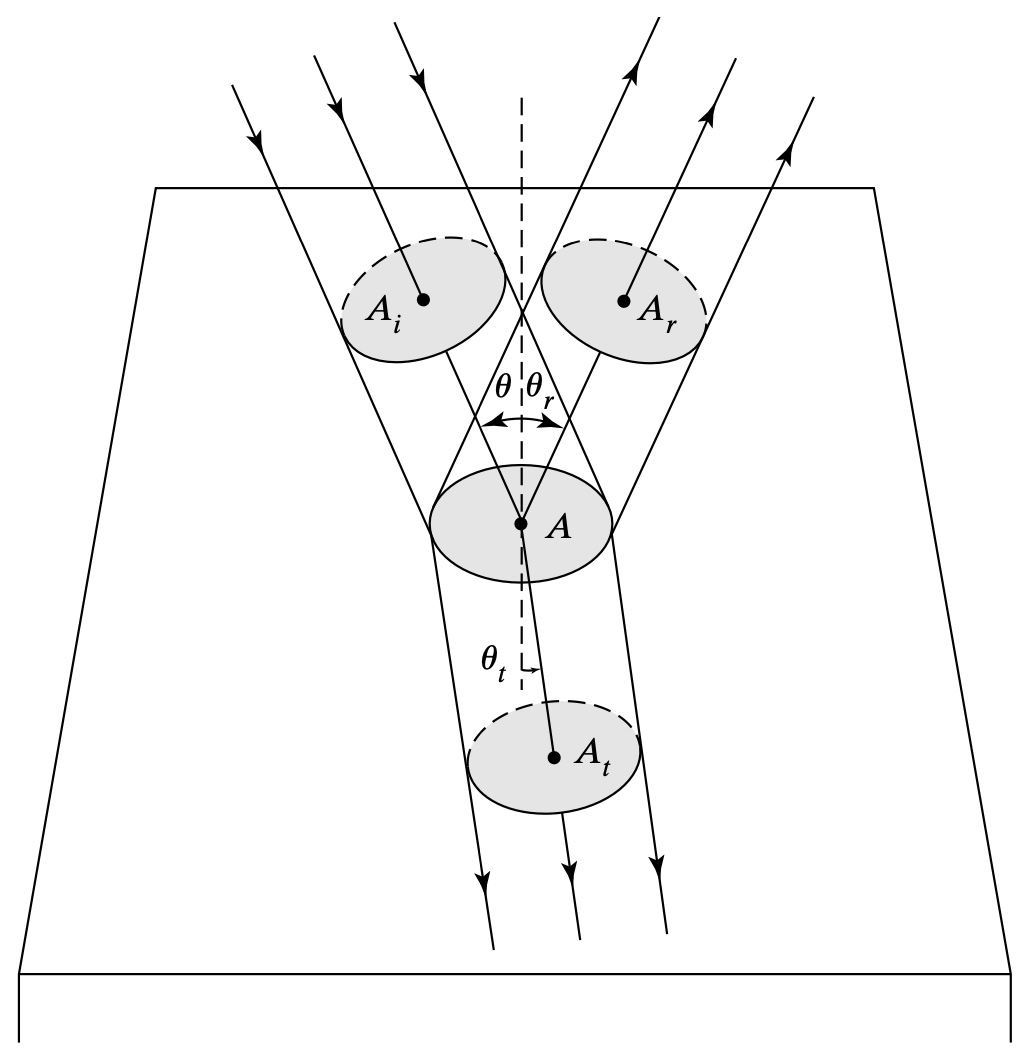
\includegraphics[width=0.8\textwidth]{Chapters/Figures/Chapter 2 Figures/CSA Example for the Incident, Reflected, and Transmitted Electromagnetic Waves.jpg}
  \caption[Cross sections of the incident, reflected, and transmitted beams]{Cross sections of the incident, reflected, and transmitted beams. Source: \cite{pedrotti_introduction_2007}}
  \label{fig: The CSA Example}
\end{figure}

Using the relation between irradiance and electrical field amplitude, 
\begin{equation}\label{eq: definition of irradiance}
I = E_{0}^2(\frac{\varepsilon \nu}{2})
\end{equation}
where:
\begin{itemize}
    \item $I$ represents the irradiance, which is the power per unit area received by a surface
    \item $E_0$ is the amplitude of the electric field, indicating the maximum strength of the field.
    \item $\varepsilon$ denotes the permittivity of the medium.
    \item $\nu$ is the phase velocity of the electromagnetic wave in the medium.
\end{itemize}
and that $\nu_i = \nu_r$ and $\varepsilon_i = \varepsilon_r$ since they correspond to the same medium, we can rephrase the power balance equation to be:
\begin{equation}
E_{0i}^2 = E_{0r}^2 + E_{0t}^2\left(\frac{\nu_t\varepsilon_t}{\nu_i\varepsilon_i}\right) \left(\frac{cos(\theta_t)}{cos(\theta)} \right)
\end{equation}
where
\begin{itemize}
    \item $E_{0i}$, $E_{0r}$, and $E_{0t}$ represent the electric field amplitudes of the incident, reflected, and transmitted waves, respectively.
    \item $\nu_i$ and $\nu_r$ denote the phase velocities in the incident and reflected paths, which are equal since these paths are within the same medium.
    \item $\varepsilon_i$ and $\varepsilon_r$ are the permittivities of the medium for the incident and reflected waves, equal because they pertain to the same medium.
    \item $\nu_t$ and $\varepsilon_t$ refer to the phase velocity and permittivity in the transmission path, respectively.
    \item The angles $\theta$ and $\theta_t$ are the angles of incidence and transmission, respectively.
\end{itemize}

The ratio $\frac{\nu_t\varepsilon_t}{\nu_i\varepsilon_i}$ is a complicated way of expressing $n$ - the relative refractive index. Considering that $\mu_i = \mu_t = \mu_0$ for nonmagnetic materials, where $\mu_i$ and $\mu_t$ are the magnetic permeabilities of the incident and transmitted materials, and $\mu_0$ is the magnetic permeability of free space. The relationship, $\nu^2 = \frac{1}{\mu \varepsilon}$ further elucidates the link between phase velocity, magnetic permeability, and permittivity. Hence, we derive:
\begin{equation}
\frac{\nu_t\varepsilon_t}{\nu_i\varepsilon_i} = \frac{\nu_i^2\mu_i}{\nu_t^2\mu_t} \frac{\nu_t}{\nu_i} = \frac{\nu_i}{\nu_t} = n
\end{equation}
This transformation streamlines the comprehension of how waves interact with various media by introducing the concept of the relative refractive index, $n$. This index represents the ratio of the phase velocities of the wave as it moves from the incident to the transmitted medium, thus quantifying the change in phase speed resulting from the passing of the wave between these two media.

Thus we can include $n$ in the power balance equations:
\begin{equation}
E_{0i}^2 = E_{0r}^2 + n E_{0t}^2 \left(\frac{cos(\theta_t)}{cos(\theta)} \right)
\end{equation}
Dividing through by $E_{0i}^2$, we get:
\begin{equation} \label{power balance equation with r^2 and t^2}
1 = r^2 + n t^2 \left(\frac{cos(\theta_t)}{cos(\theta)} \right)
\end{equation}
% Note that equations \ref{Definition of the reflection coefficient} and \ref{Definition of the transmission coefficient} allow us to make the substitutions for $r$ and $t$ above. Note that \ref{power balance equation with r^2 and t^2} certify that:

Reflectance ($R$) and transmittance ($T$) quantify the fractions of incident electromagnetic power that are reflected and transmitted across a boundary, respectively. These concepts are grounded in the principle of energy conservation, which, in the context of electromagnetic waves at an interface, is expressed as:
\begin{equation}
    R = \frac{P_r}{P_i} = \frac{I_r}{I_i} = \left(\frac{E_{0r}}{E_0i}\right)^2 = r^2
\end{equation}
where in the last step, I have utilized equation \ref{eq: definition of irradiance}. The term $r^2$ is introduced as a shorthand notation for this ratio, encapsulating the reflectance in terms of the electric field amplitude rations.

Looking at equation \ref{R+T=1}, we gather that:
\begin{equation} \label{definition of T}
T =  n t^2 \left(\frac{cos(\theta_t)}{cos(\theta)} \right)
\end{equation}

It's worth noting that $T$ is not merely $t^2$, as we must consider the altered speed of the electromagnetic wave when it enters a medium with a different refractive index. This change in speed impacts the rate of energy propagation and, consequently, the power of the beam.

\begin{figure}[ht!]
  \centering
  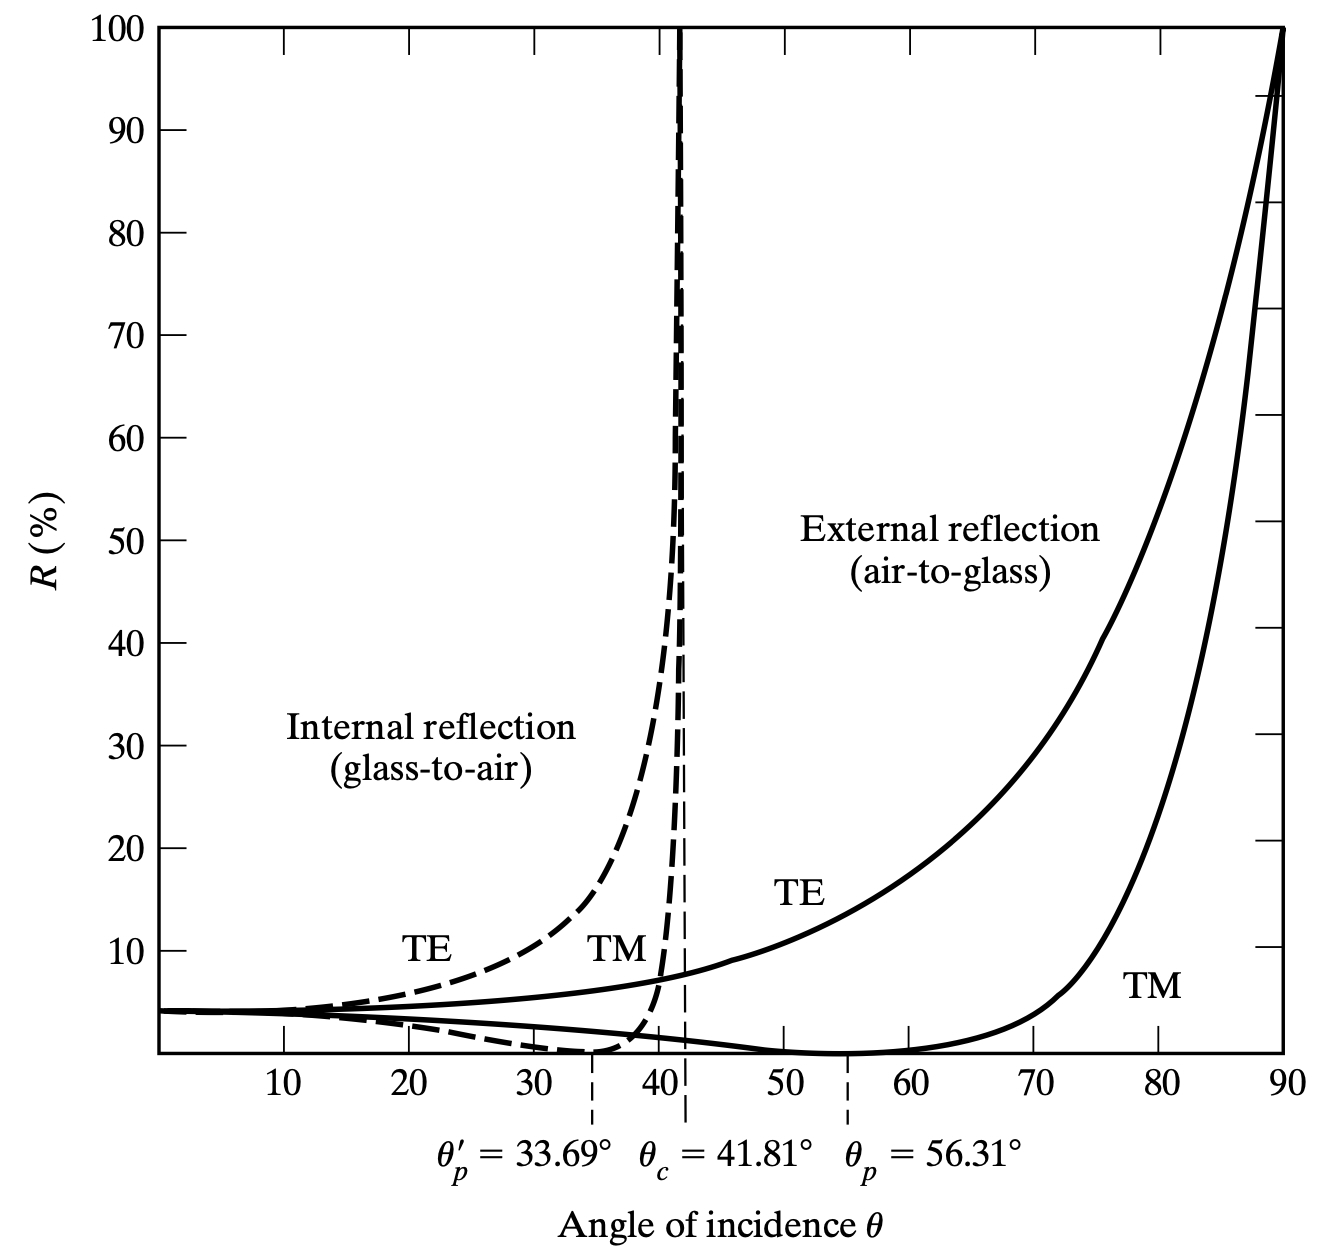
\includegraphics[width=0.6\textwidth]{Chapters/Figures/Chapter 2 Figures/Reflectance vs Angle of Incidence.jpg}
  \caption[Reflectance vs Angle of Incidence]{Reflectance vs Angle of Incidence. Source: \cite{pedrotti_introduction_2007}}
  \label{fig: R vs Theta}
\end{figure}

Figure \ref{fig: R vs Theta} illustrates how the reflectance $R$ of light varies with the angle of incidence $\theta$ for two different polarizations of light we've looked at, the transverse electric (TE) and transverse magnetic (TM). The graph is split into two regions that represent different physical scenarios of light interaction with a boundary: internal reflection (glass-to-air) and external reflection (air-to-glass).

The critical angle, denoted as $\theta_c$, represents the specific angle of incidence at which a refracted light ray grazes the interface between two media. At this angle, the ray runs parallel to the boundary, without penetrating into the second medium or retreating into the first. When the angle of incidence surpasses $\theta_c$, a scenario of total internal reflection unfolds: all the incident light is entirely reflected into the originating denser medium, and no light is refracted into the less dense medium, such as air. This results in the graph indicating a reflectance of 100\% for both TE and TM polarization states in situations of glass-to-air transition. This effect is exclusive to internal reflection; conversely, when light travels from a less dense to a denser medium, it is almost always refracted into the denser medium, a behavior consistent across all incidence angles.

Brewster's Angles, marked by vertical dashed lines at \(56.31^\circ\) for external reflection (air-to-glass) and \(33.69^\circ\) for internal reflection (glass-to-air), correspond to the specific angles of incidence where the reflectance reaches a minimum for TM-polarized light in external reflection and internal reflection respectively. At these angles, the reflected intensity is significantly reduced for the respective polarization states.

$n$ is a function of the wavelength ($\lambda$) of light. Consequently, both reflectance ($R$) and transmittance ($T$) are wavelength-dependent. This wavelength dependence is particularly relevant to the scope of this work as it influences the behavior of light across different spectra. The refractive index’s variation with wavelength means that the critical and Brewster's angles, and therefore the efficiency of reflection and transmission, will vary with the wavelength of the incident light, which has significant implications for applications that rely on precise control of light propagation, such as in optical filters and coatings.

%------------- FROM THE THEORY OF MULTILAYER FILMS ------------
\section{Multilayer films}
In the development of Passive Daytime Radiative Cooling Devices (PDRCs), we intend to employ multiple stacks comprising diverse materials with distinct refractive indices, arranged in layers to enhance the overall reflection coefficient and consequently increase reflectance. It is crucial to comprehend the electromagnetic wave interaction and optimal layer stacking physics to maximize reflectance. We again need a rigorous consideration of boundary conditions as dictated by Maxwell's equations.

%------------- TRANSFER MATRIX SECTION ------------
\subsection{Transfer Matrix}
Consider the set-up above where the electric field amplitude is perpendicular to the plane of incidence (a transverse electric (TE) wave).

% inserting the multilayer film set-up
\begin{figure}
  \centering
  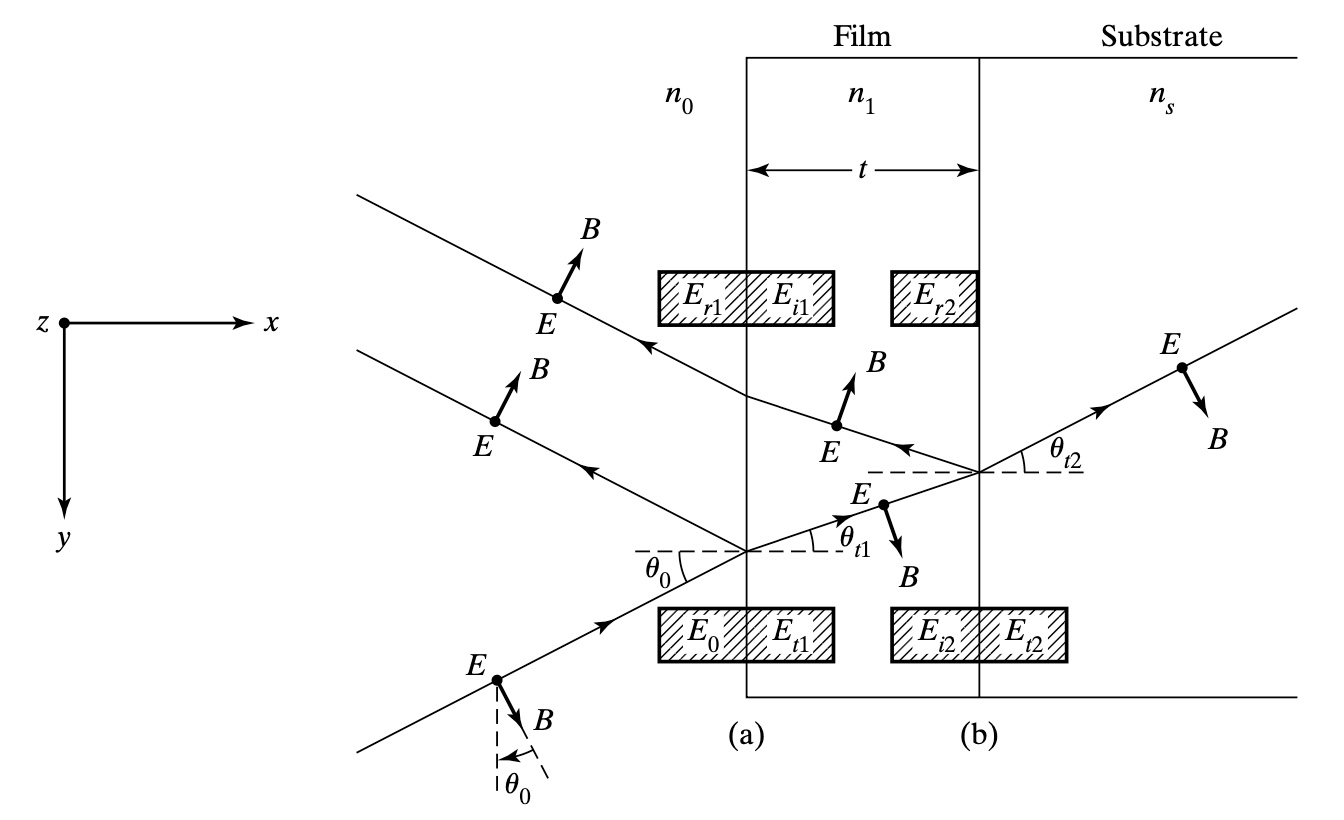
\includegraphics[width=0.8\textwidth]{Chapters/Figures/Multilayer Film Set-Up.jpeg}
  \caption{Multilayer Film Set-Up}
\end{figure}

A TE wave propagates from air, reaching the air-film boundary. A fraction of the wave is transmitted, while another portion is reflected. The transmitted portion encounters the film-substrate interface, where part is further transmitted, and another part is reflected. This reflected component then becomes incident on the film-air interface, leading to transmission and reflection, repeating the process. This scenario can be extrapolated to involve multiple films. It is important to note that the film and substrate possess distinct refractive indices, denoted as $n_1$ and $n_s$ respectively. %R

To capture the complex interaction between reflected and transmitted beams, we employ a systematic notation, as seen in the provided setup image. For example, $E_{r1}$ denotes the aggregate of multiply reflected beams at interface (a), while $E_{i2}$ signifies the sum of multiple incident beams at interface (b), directed toward the substrate. %R

Again, we hold true to our assumptions that the film is both homogeneous (has the same properties at every point) and isotropic (the physical properties do not differ regardless of the direction or orientation in which it is examined). Moreover, we assume further that the thickness of the film is on the order of wavelength of light.

The boundary conditions derived from Maxwell's equations stipulate that the tangential components of the electric and magnetic fields in plane waves must exhibit continuity across the interface, remaining equal on both sides. It is essential to recognize that while the electric field component is tangential to the interfaces everywhere, the orthogonal nature of the magnetic field vector to the electric field vector necessitates the determination of corresponding tangential magnetic field vectors. This endeavor aims to establish a formula that correlates the electric and magnetic fields at one interface with those at the subsequent interface. %R

    \begin{equation} \label{E_a - Multilayer films electric field boundary equations}
    E_a = E_0 + E_{r1} = E_{t1} + E_{i1}
    \end{equation}
    
    \begin{equation} \label{E_b - Multilayer films electric field boundary equations}
    E_b = E_{i2} + E_{r2} = E_{t2}
    \end{equation}

To determine the tangential magnetic field vectors, trigonometry can be applied to establish the following boundary conditions:

    \begin{equation} \label{B_a - Multilayer films magnetic field boundary equations}
    B_a = B_0cos(\theta_0) - B_{r1}cos(\theta_0) = B_{t1}cos(\theta_{t1}) - B_{i1}cos(\theta_{t1})
    \end{equation}

    \begin{equation} \label{B_b - Multilayer films magnetic field boundary equations}
    B_b = B_{i2}cos(\theta_{t1}) - B_{r2}cos(\theta_{t1}) = B_{t2}cos(\theta_{t2})
    \end{equation}

We can build on equation \ref{Equation relating the electric and magnetic field amplitudes} by expressing B in terms of E as:
    \begin{equation} \label{Alternative B and E representation}
    B = n\sqrt{\varepsilon_0\mu_0}E
    \end{equation}
and since $c=\frac{1}{\sqrt{\varepsilon_0\mu_0}}$, we can rewrite \ref{B_a - Multilayer films magnetic field boundary equations} and \ref{B_b - Multilayer films magnetic field boundary equations} employing \ref{Alternative B and E representation}.

    \begin{equation} \label{Alternative B_a - Multilayer films magnetic field boundary equations}
    B_a = \gamma_0(E_0 - E_{r1}) = \gamma_1(E_{t1} - E_{i1})
    \end{equation}

    \begin{equation} \label{Alternative B_b - Multilayer films magnetic field boundary equations}
    B_b = \gamma_1(E_{i2} - E_{r2}) = \gamma_sE_{t2}
    \end{equation}
where
    % -- THE GAMMA EQUATIONS --
    \begin{equation} \label{gamma 0}
        \gamma_0 \equiv n_0 \sqrt{\varepsilon_0\mu_0} cos(\theta_0)
    \end{equation}

    \begin{equation} \label{gamma 1}
        \gamma_1 \equiv n_1 \sqrt{\varepsilon_0\mu_0} cos(\theta_{t1})
    \end{equation}

    \begin{equation} \label{gamma s}
        \gamma_s \equiv n_s \sqrt{\varepsilon_0\mu_0} cos(\theta_{t2})
    \end{equation}

% I NEED TO LOOK MORE INTO THE OPTICAL PATH LENGTH TO OFFER A BETTER EXPLANATION l
$E_{i2}$ differs from $E_{t1}$ solely due to a phase difference $\delta$ arising from a single traversal of the film. The optical path length linked with one traversal is denoted as $\Delta_1=n_1t\cos(\theta_{t1})$. The optical path length represents the distance that light "perceives" it has covered in a medium and can be quantified in terms of the number of cycles the light beam has undergone within that specific medium. It is inherently proportional to the refractive index and the geometric length of the medium through which light is propagating. %R

We can express the phase difference that develops due to one traversal of the film as:
    \begin{equation} \label{phase difference}
    \delta = k_0\Delta_1 = \left(\frac{2\pi}{\lambda_0}\right) n_1tcos(\theta_{t1})
    \end{equation}

Therefore we can express the pair electric field sums $E_{i2}$ \& $E_{t1}$ and $E_{i1}$ \& $E_{r2}$ as follows:
    \begin{align*}
        E_{i2} = E_{t1}e^{-i\delta} \\
        E_{i1} = E_{r2}e^{-i\delta}
    \end{align*}
and consequently rephrase \ref{E_b - Multilayer films electric field boundary equations} and \ref{Alternative B_b - Multilayer films magnetic field boundary equations} as:

    \begin{equation} \label{E_b form after phase difference}
    E_b = E_{t1}e^{-i\delta} + E_{i1}e^{i\delta} = E_{t2}
    \end{equation}
    
    \begin{equation} \label{B_b form after phase difference}
    B_b = \gamma_1(E_{t1}e^{-i\delta} - E_{i1}e^{i\delta}) = \gamma_sE_{t2}
    \end{equation}

Looking at the middle terms, we can solve for $E_{t1}$ and $E_{i1}$ in terms of $E_b$ and $B_b$.
    \begin{equation} \label{E_t1}
    E_{t1} = \left(\frac{\gamma_1E_b + B_b}{2\gamma_1}\right)e^{i\delta}
    \end{equation}
    
    \begin{equation} \label{E_i1}
    E_{i1} = \left(\frac{\gamma_1E_b - B_b}{2\gamma_1}\right)e^{-i\delta}
    \end{equation}

Utilizing the Euler identities $2isin(\delta) \equiv e^{i\delta} - e^{-i\delta}$ and $2cos(\delta) \equiv e^{i\delta} + e^{-i\delta}$, we can use the equations \ref{E_t1} and \ref{E_i1} and substitute them into \ref{E_a - Multilayer films electric field boundary equations} and \ref{Alternative B_b - Multilayer films magnetic field boundary equations} to have both:

    \begin{equation} \label{E_a in terms of E_b and B_b}
    E_a = E_bcos(\delta) + B_b\left(\frac{isin(\delta)}{\gamma_1}\right)
    \end{equation}
    
    \begin{equation} \label{B_a in terms of E_b and B_b}
    B_a = E_b(i\gamma_1sin(\delta)) + B_bcos(\delta)
    \end{equation}
which we can rewrite in matrix notation as:

% I don't know why this works but I will not mess with it
    \[
      \begin{bmatrix}\label{Full form transfer matrix}
        E_a  \\
        B_a
      \end{bmatrix} = 
        % \[
            \begin{bmatrix}
            cos(\delta) & \frac{isin(\delta)}{\gamma_1}    \\
            i\gamma_1sin(\delta) & cos(\delta)
            \end{bmatrix}
        % \[
            \begin{bmatrix}
            E_b  \\
            B_b
          \end{bmatrix}
        % \]
        % \]
    \]

This notation introduces the insightful $2 \times 2$ matrix that establishes a connection between the electric and magnetic fields at one interface and those at the subsequent interface. Termed the \emph{transfer matrix}, we will refer to this significant matrix in a generic manner as: %R
    \[
    M=
      \begin{bmatrix}
        m_{11} & m_{12}  \\
        m_{21} & m_{22}
      \end{bmatrix}
    \]

Expanding this framework, we can extend the consideration to the stacking of multiple films, leading to the emergence of multiple interfaces. In a more general context, for an arbitrary number N of layers: %R
    \[
      \begin{bmatrix}
        E_a  \\
        B_a
      \end{bmatrix} = 
        % \[
            M_1M_2M_3\hdots M_N
        % \[
            \begin{bmatrix}
            E_N \\
            B_N
          \end{bmatrix}
        % \]
        % \]
    \]
with the multiplication of individual transfer matrices representing the entire multilayer stack in the order in which the beam encounters them.

Returning to the comprehensive form of the transfer matrix presented above, we can substitute $E_a$ and $B_a$ with the middle segments of equations \ref{E_a - Multilayer films electric field boundary equations} and \ref{Alternative B_a - Multilayer films magnetic field boundary equations}. Similarly, $E_b$ and $B_b$ can be replaced with the rightmost segments of equations \ref{E_b form after phase difference} and \ref{B_b form after phase difference}, resulting in: %R
    \[
      \begin{bmatrix}
        E_0 + E_{r1}  \\
        \gamma_0(E_0 - E_{r1})
      \end{bmatrix} = 
        % \[
            \begin{bmatrix}
            cos(\delta) & \frac{isin(\delta)}{\gamma_1} \\
            i\gamma_1sin(\delta) & cos(\delta)
            \end{bmatrix}
        % \[
            \begin{bmatrix}
            E_{t2}  \\
            \gamma_sE_{t2}
          \end{bmatrix} =
          % \[
                \begin{bmatrix}
                    m_{11} & m_{12} \\
                    m_{21} & m_{22}
                \end{bmatrix}
                % \[
                \begin{bmatrix}
                    E_{t2} \\
                    \gamma_sE_{t2}
                  \end{bmatrix}
                % \]
          % \]
        % \]
        % \]
    \]

Recall $r \equiv \frac{E_{r1}}{E_0}$ and $t \equiv \frac{E_{t2}}{E_0}$ (the reflection and transmission coefficients, respectively). By matrix multiplication, we can simplify the resulting equation to obtain: %R
    \begin{equation}
    1 + r = m_{11}t + m_{12}\gamma_st
    \end{equation}
    \begin{equation}
    \gamma_0(1 - r) = m_{21}t + m_{22}\gamma_st
    \end{equation}

Solving for $r$ by solving the system of linear equations above, we get
    \begin{equation}\label{reflection coefficient in terms of transfer matrix terms}
    r=\frac{\gamma_0m_{11} + \gamma_0\gamma_sm_{12} - m_{21} - \gamma_sm_{22}}{\gamma_0m_{11} + \gamma_0\gamma_sm_{12} + m_{21} + \gamma_sm_{22}}
    \end{equation}

%----- SECTION OF ANTIREFLECTING FILMS -------
\subsection{Antireflecting Films}
To gain a deeper insight into optimizing reflectance, let's explore the characteristics conducive to antireflection. Employing a double layer of quarter-wave-thickness films allows for the attainment of minimal reflectance at a specific wavelength. We will examine the simplest scenario for normal incidence, where all angles of incidence, reflection, and refraction are zero. The corresponding transfer matrix is expressed as: %R

    \[
    M = 
        % \[
            \begin{bmatrix}
            cos(\delta) & \frac{isin(\delta)}{\gamma_1} \\
            i\gamma_1sin(\delta) & cos(\delta)
            \end{bmatrix} = 
            % \[
                \begin{bmatrix}
                0 & \frac{i}{\gamma_1}  \\
                i\gamma_1 & 0
              \end{bmatrix}
            % \]
        % \]
    \]
since, at quarter-wave thickness, $t=\frac{\lambda}{4} = \frac{1}{4} \times \frac{\lambda_0}{n_1} = \frac{\lambda_0}{4n_1}$. Recall also we defined the phase difference, \ref{phase difference}, to be
    \begin{align*}
        \delta &= \left(\frac{2\pi}{\lambda_0}\right) n_1tcos(\theta_{t1})\\
        \delta &= \left(\frac{2\pi}{\lambda_0}\right) n_1tcos(0) \\
        \delta &= \left(\frac{2\pi}{\lambda_0}\right) n_1t\\
        \delta &= \frac{\pi}{2} \\
    \end{align*}
so that $cos(\delta) = 0$ and $sin(\delta) = 1$.

For two quarter-wave thickness films of similar form, the overall transfer matrix can be obtained by multiplying the individual transfer matrices:
    \[
    M = 
        % \[
            \begin{bmatrix}
            -\frac{\gamma_2}{\gamma_1} & 0 \\
            0 & -\frac{\gamma_1}{\gamma_2}
          \end{bmatrix}
        % \]
    \]

Equation \ref{reflection coefficient in terms of transfer matrix terms}, the reflection coefficient, then simplifies to:
    \begin{equation}\label{reflection coefficient for 2-layer antireflecting films}
    r = \frac{\gamma_2^2\gamma_0 - \gamma_s\gamma_1^2}{\gamma_2^2\gamma_0 + \gamma_s\gamma_1^2}
    \end{equation}

The reflectance, $R$, is simply $|r|^2$ and using equations \ref{gamma 0} through \ref{gamma s}, we can calculate $R$ to be
    \begin{equation}\label{reflectance for 2-layer antireflecting films}
    R = \left(\frac{n_0n_2^2 - n_sn_1^2}{n_0n_2^2 + n_sn_1^2}\right)^2
    \end{equation}

Zero reflectance is then expected when the numerator is zero
    \begin{align*}
        n_0n_2^2 = n_sn_1^2 \\
        \frac{n_2^2}{n_1^2} = \frac{n_s}{n_0}  \\
    \end{align*} so that
    \begin{equation}\label{zero reflectance criterion}
    \frac{n_2}{n_1} = \sqrt{\frac{n_s}{n_0}}
    \end{equation}

For a glass substrate with a refractive index of $n_s = 1.52$ and incidence from air with $n_0 = 1$, the optimal ratio of the refractive indices for the two films should be $\frac{n_2}{n_1} = \sqrt{1.52} = 1.23$. However, achieving near-zero reflectance is challenging over the broader region of the visible spectrum.

\begin{figure}
  \centering
  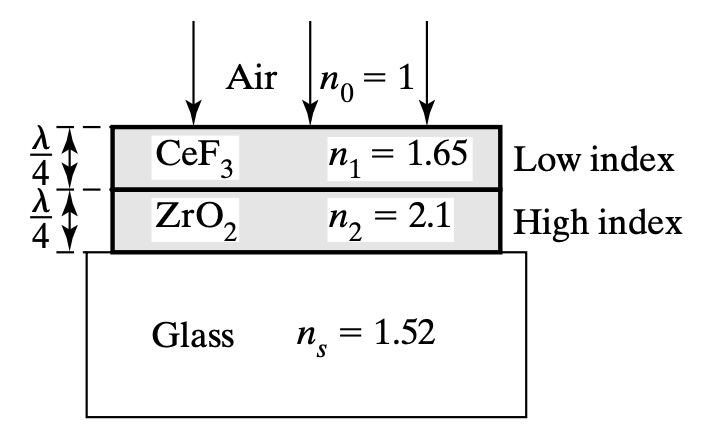
\includegraphics[width=0.4\textwidth]{Chapters/Figures/Antireflecting Double Layer.jpeg}
  \caption{Antireflecting Double Layer}
\end{figure}

PERSONAL NOTE - I WILL INCLUDE A FIGURE OF REFLECTANCE VERSUS WAVELENGTH ONCE I GENERATE THE STUDY ON COMSOL.

%----- SECTION ON HIGH-REFLECTANCE LAYERS -------
\subsection{High-Reflectance Layers.}
In the previous section, we established that to optimize for anti-reflectance, we stack layers in the order of air-low index-high index-substrate. Conversely, to optimize for high-reflectance, we follow the opposite order: air-high index-low index-substrate. A set of double layers designed to enhance reflectance is referred to as a \emph{high-reflectance stack} or \emph{dielectric mirror}. %R

PERSONAL NOTE - I WILL INCLUDE A FIGURE OF REFLECTANCE VERSUS WAVELENGTH ONCE I GENERATE THE STUDY ON COMSOL.

The transfer matrix for the two films in the order of high index-low index is
    \[
      M_{HL} = 
        % \[
            \begin{bmatrix}
            0 & \frac{i}{\gamma_H} \\
            i\gamma_H & 0
            \end{bmatrix}
        % \[
            \begin{bmatrix}
            0 & \frac{i}{\gamma_L} \\
            i\gamma_L & 0
            \end{bmatrix} =
                % \[
                    \begin{bmatrix}
                        -\frac{\gamma_L}{\gamma_H} & 0  \\
                        0 & -\frac{\gamma_H}{\gamma_L}
                    \end{bmatrix}
                % \]
        % \]
        % \]
    \]
    
For N similar double layers, we obtain $M = (M_{HL})^N$. In matrix form,
    \[
      M = 
        % \[
            \begin{bmatrix}
            0 & \frac{i}{\gamma_L} \\
            i\gamma_L & 0
            \end{bmatrix}^N =
          % \[
                \begin{bmatrix}
                    \left(-\frac{\gamma_L}{\gamma_H}\right)^N & 0  \\
                    0 & \left(-\frac{\gamma_H}{\gamma_L}\right)^N
                \end{bmatrix}
        % \]
        % \]
        % \]
    \]

Considering normal incidence and using equations \ref{gamma 0} through \ref{gamma s},
    \begin{align*}
        \frac{\gamma_L}{\gamma_H} &= \frac{n_L\sqrt{\varepsilon_0\mu_0}cos(\frac{\pi}{2})}{n_H\sqrt{\varepsilon_0\mu_0}cos(\frac{\pi}{2})}\\
        \frac{\gamma_L}{\gamma_H} &= \frac{n_L\sqrt{\varepsilon_0\mu_0}}{n_H\sqrt{\varepsilon_0\mu_0}}  \\
        \frac{\gamma_L}{\gamma_H} &= \frac{n_L}{n_H}
    \end{align*}
Similarly, $\frac{\gamma_H}{\gamma_L} = \frac{n_H}{n_L}$

Equation \ref{reflection coefficient in terms of transfer matrix terms}, the reflection coefficient, then simplifies to:
    \begin{equation}\label{reflection coefficient for double high-reflectance layers}
    r = \frac{n_0\left(\frac{-n_L}{n_H}\right)^N - n_s\left(\frac{-n_H}{n_L}\right)^N}{n_0\left(\frac{-n_L}{n_H}\right)^N + n_s\left(\frac{-n_H}{n_L}\right)^N}
    \end{equation}

To get $R$, we calculate $|r|^2$ to get
    \begin{equation}\label{maximum reflectance equation}
    R = \left[ \frac{ \left( \frac{n_0}{n_s} \right) \left( \frac{n_L}{n_H} \right)^{2N}  - 1 }{  \left( \frac{n_0}{n_s} \right) \left( \frac{n_L}{n_H} \right)^{2N}  + 1     }  \right]^2
    \end{equation}
PERSONAL NOTE - ONCE I FIGURE HOW TO DO SO, I SHALL INCLUDE THE STEPS IN THE DERIVATION OF \ref{maximum reflectance equation}.

Maximum (100\%) reflectance is either achieved when:
    \begin{enumerate}
      \item When $N$ approaches infinity.
      \item When $\frac{n_L}{n_H}$ approaches zero. For example, when this ratio is 0.5 and there are 3 layers, a reflectance of 95.97 is achieved.
    \end{enumerate}
Since the optimal reflectance is obtained with the smallest ratio of $\frac{n_L}{n_H}$, high-reflectance stacks can be constructed using alternating layers of $MgF_2$ $(n_L = 1.38$) and $ZnS$ $(n_H = 2.35)$ or $TiO_2$ $(n_H = 240)$. For example, employing alternating double layers of $MgF_2$ and $ZnS$ can achieve a reflectance of 99.95\% with a layer count ($N$) of 8. %R

PERSONAL NOTE - I WILL INCLUDE A FIGURE OF THE SPECTRAL REFLECTANCE OF A HIGH-LOW INDEX STACK ONCE I GENERATE IT ON COMSOL.
